\chapter{DFA::min\_Hopcroft() 的扩展测试}
本文对 DFA::min\_Hopcroft 算法的更改进行测试对比说明。由代码 \ref{list:hop} 更改为代码 \ref{list:hopedit}
\lstset{style=mystyle}
\begin{lstlisting}[language=c++,label={list:hop},caption={原始的 Hopcroft}]
    // mark this element of L as processed. ([q],c)
    L[q]--;

    // Iterate over all eq. classes, and try to split them.
    State p;
    repr = P.representatives(); // all partitions(eq.classes)
    for (repr.iter_start(p); !repr.iter_end(p); repr.iter_next(p))
    {
        // Now split [p] w.r.t (q, C_(L[q]))
        State r(split(p, q, C.iterator(L[q]), P)); 
\end{lstlisting}

%\lstset{style=mystyle}
\begin{lstlisting}[language=c++,label={list:hopedit},caption={更改后的 Hopcroft}]
    // mark this element of L as processed. ([q],c)
    L[q]--;
    CharRange c = C.iterator(L[q]); // 记录正在处理的c      //新增位置

    // Iterate over all eq. classes, and try to split them.
    State p;
    repr = P.representatives(); // all partitions(eq.classes)
    for (repr.iter_start(p); !repr.iter_end(p); repr.iter_next(p))
    {
        // Now split [p] w.r.t (q, C_(L[q]))
        State r(split(p, q, c, P));                       //更改位置
\end{lstlisting}


\begin{figure}[!htbp]
    \centering
    \begin{subfigure}[b]{0.49\textwidth}
        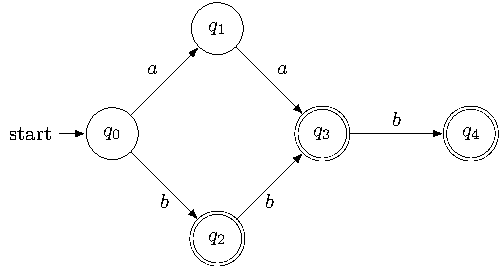
\includegraphics[width=\textwidth]{keepMin/hoperror--1}
        \caption{$\mathcal{L}=\{aa \cup aab \cup b \cup bb \cup bbb\}$}
        \label{fig:hoperror--1}
    \end{subfigure}
    ~
    \begin{subfigure}[b]{0.49\textwidth}
        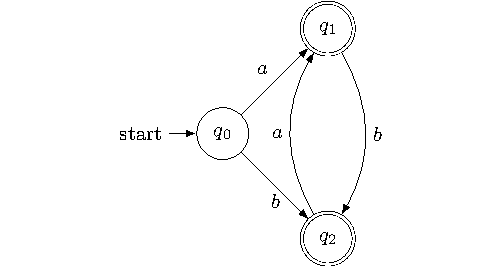
\includegraphics[width=\textwidth]{keepMin/hoperror--2}
        \caption{}
        \label{fig:hoperror--2}
    \end{subfigure}
    \\
    \begin{subfigure}[b]{0.7\textwidth}
        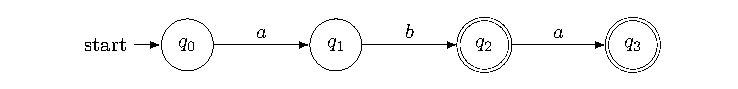
\includegraphics[width=\textwidth]{keepMin/hoperror--3}
        \caption{$\mathcal{L}=\{ab \cup aba\}$}
        \label{fig:hoperror--3}
    \end{subfigure}
    ~
    \begin{subfigure}[b]{0.7\textwidth}
        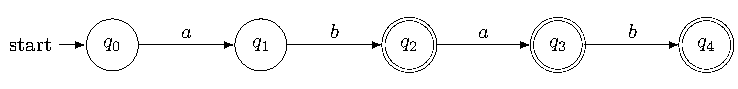
\includegraphics[width=\textwidth]{keepMin/hoperror--4}
        \caption{$\mathcal{L}=\{ab \cup aba \cup abab\}$}
        \label{fig:hoperror--4}
    \end{subfigure}
    ~
    \begin{subfigure}[b]{0.7\textwidth}
        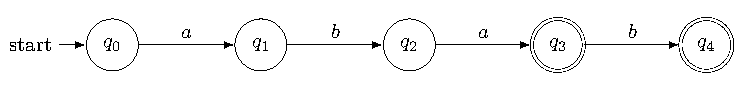
\includegraphics[width=\textwidth]{keepMin/hoperror--5}
        \caption{$\mathcal{L}=\{aba \cup abab\}$}
        \label{fig:hoperror--5}
    \end{subfigure}
    \caption{一组最小的 DFA }
    \label{fig:hopcerror}
  \end{figure}

以图 \ref{fig:hopcerror} 中的五个最小的 DFA 为数据,测试结果统计如表 \ref{tab:KeepMinResultofAll} 所示

\begin{table}[!htbp]
    \caption{  }
    \label{tab:KeepMinResultofAll}
    \centering
    \small% fontsize
    \setlength{\tabcolsep}{4pt}% column separation
    \renewcommand{\arraystretch}{1.2}%row space 
    \begin{tabular}{l|p{4em}<{\centering} p{4em}<{\centering} p{4em}<{\centering} p{4em}<{\centering} p{4em}<{\centering} }  %l p{3em}<{\centering} p{3em}<{\centering} p{3em}<{\centering}
        \toprule %\hline 
        算法 & \ref{fig:hoperror--1} & \ref{fig:hoperror--2} & \ref{fig:hoperror--3} & \ref{fig:hoperror--4} &  \ref{fig:hoperror--5}  \\
        \midrule
        DFA::min\_Brzozowski()        & $\surd$ & $\surd$ & $\surd$ & $\surd$     & $\surd$        \\
        DFA::min\_Hopcroft()(修改前) & 中止    & $\times$ & $\surd$ & 中止        & $\surd$       \\
        DFA::min\_Hopcroft()(修改后) & $\times$& $\times$& $\surd$ & $\times$    & $\surd$       \\
        DFA::min\_HopcroftUllman()    & $\surd$ & $\surd$ & $\surd$ & $\surd$     & $\surd$       \\
        DFA::min\_dragon()            & $\surd$ & $\surd$ & $\surd$ & $\surd$     & $\surd$       \\
        DFA::min\_Watson()            & $\surd$ & $\surd$ & $\surd$ & $\surd$     & $\surd$       \\
        \bottomrule%\hline  
    \end{tabular}
\end{table}

\newpage
对于图 \ref{fig:hoperror--1} ,修改后 Hopcroft 算法输出如下代码 \ref{FCode1},如图 \ref{fig:hoperror--1-result} 所示。

\begin{lstlisting}[language=bash,label={FCode1},caption={图 \ref{fig:hoperror--1} 输出}]
    DFA
    Q = [0,3)
    S = { 0 }
    F = { 2 }
    Transitions =
    0->{ 'a'->1  'b'->2 }
    1->{ 'a'->2 }
    2->{ 'b'->2 }

    current = -1
\end{lstlisting}
 
对于图 \ref{fig:hoperror--2} ,无论是否修改,Hopcroft均输出代码 \ref{FCode2},如图 \ref{fig:hoperror--2-result} 所示。
\begin{lstlisting}[language=bash,label={FCode2},caption={图 \ref{fig:hoperror--2} 输出}]
    DFA
    Q = [0,2)
    S = { 0 }
    F = { 1 }
    Transitions =
    0->{ ['a','b']->1 }
    1->{ 'b'->1 }

    current = -1
\end{lstlisting}

对于图 \ref{fig:hoperror--4} , 修改后 Hopcroft 输出代码 \ref{FCode4},如图 \ref{fig:hoperror--4-result} 所示。
\begin{lstlisting}[language=bash,label={FCode4},caption={图 \ref{fig:hoperror--4} 输出}]
    DFA
    Q = [0,3)
    S = { 0 }
    F = { 2 }
    Transitions =
    0->{ 'a'->1 }
    1->{ 'b'->2 }
    2->{ 'a'->2 }

    current = -1
\end{lstlisting}


\begin{figure}[!htbp]
    \centering
    \begin{subfigure}[b]{0.7\textwidth}
        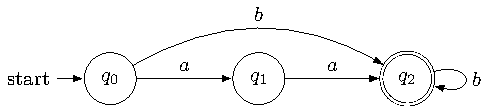
\includegraphics[width=\textwidth]{keepMin/hoperror--1-result}
        \caption{$\mathcal{L}=\{aa(b)^* \cup b(b)^*\}$}
        \label{fig:hoperror--1-result}
    \end{subfigure}
    \\
    %\vfill% \vspace{1cm}
    \begin{subfigure}[b]{0.7\textwidth}
        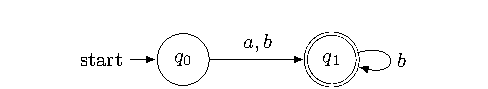
\includegraphics[width=\textwidth]{keepMin/hoperror--2-result}
        \caption{$\mathcal{L}=\{a(b)^* \cup b(b)^*\}$}
        \label{fig:hoperror--2-result}
    \end{subfigure}
    \\
    %\vfill% \vspace{1cm}
    \begin{subfigure}[b]{0.7\textwidth}
        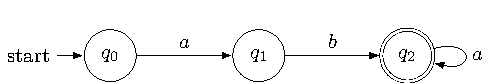
\includegraphics[width=\textwidth]{keepMin/hoperror--4-result}
        \caption{$\mathcal{L}=\{ab(a)^*\}$}
        \label{fig:hoperror--4-result}
    \end{subfigure}
    \caption{Hopcroft 算法的输出 }
    \label{fig:hopcerror-result}
  \end{figure}

  表 \ref{tab:KeepMinResultofAll-hop} 为对比数据

  \begin{table}[!htbp]
    \caption{  }
    \label{tab:KeepMinResultofAll-hop}
    \centering
    \small% fontsize
    \setlength{\tabcolsep}{4pt}% column separation
    \renewcommand{\arraystretch}{1.2}%row space 
    \begin{tabular}{c p{2em}<{\centering}p{2em}<{\centering}ccc }  %l p{3em}<{\centering} p{3em}<{\centering} p{3em}<{\centering}
        \toprule %\hline 
        数据 & $|Q|$ & $|F|$ & $|F|\leq |Q \setminus F|$? & 修改前结果 &  修改后结果  \\
        \midrule
        图 \ref{fig:hoperror--1}        & 5 & 3 & 否 & 中止       & $\times$        \\
        图 \ref{fig:hoperror--2}        & 3 & 2 & 否 & $\times$   & $\times$       \\
        图 \ref{fig:hoperror--3}        & 4 & 2 & 是 & $\surd$    & $\surd$       \\
        图 \ref{fig:hoperror--4}        & 5 & 3 & 否 & 中止       & $\times$       \\
        图 \ref{fig:hoperror--5}        & 5 & 2 & 是 & $\surd$    & $\surd$       \\
        \bottomrule%\hline  
    \end{tabular}
\end{table}

% 图 fig:hopcerror 中的数据在除 Hopcroft 之外的算法的测试中通过,所以本文认为 FIRE engine 对 Hopcroft 算法的实现仍有不足

%l|p{4em}<{\centering} p{4em}<{\centering} p{4em}<{\centering} p{4em}<{\centering} p{4em}<{\centering}